
\label{sec:model} 
%We define here a hierarchically supervised LDA
%model. Although we will focus on document modeling in our description
%and experiments, this model applies equally well to other collections
%of discrete data with hierarchically constrained labels. 

HSLDA is a model for hierarchically, multiply-labeled, bag-of-words data.  We will refer to individual groups of bag-of-word data as documents.  Let $w_{n,d} \in \Sigma$ be the $n$th observation in the $d$th document.  Let $\mathbf{w}_d = \{w_{1,d},\ldots,w_{1,N_d}\}$ be the  set of $N_d$ observations in document $d$.  Let there be $D$ such documents and let the size of the vocabulary be $V=|\Sigma|$.  Let the set of labels be $\mathcal{L}=\left\{ l_{1},l_{2},\ldots,l_{\left|\mathcal{L}\right|}\right\} $. Each label $l \in \mathcal{L}$ has a parent $\mathrm{pa}(l) \in \mathcal{L}$ also in the set of labels.
 We will for exposition purposes assume that this label set has hard ``is-a'' parent-child constraints (explained later), although this assumption can be relaxed at the cost of more complicated inference.  Such a label hierarchy forms a multiply rooted tree.  Without loss of generality we will consider a trees with a single root $r\in\mathcal{L}$.  Each document has a response $y_{l,d} \in \{-1,1\}$ to every label which indicates whether the label applies to document $d$ or not.  
 
 
The is-a hierarchical constraint is a hard constraint that 
document $d$ has a positive response
to label $l_{2}$ then it will also have a positive response to label
$l_{1}$. Conversely, if document $d$ has a negative response to
label $l_{1}$ then it will also has a negative response to $l_{2}$.
To capture this hierarchical structure we model the labeling of documents
using a generative cascade of conditional probit regression models.


Each document is assigned a response of either -1 or 1 for at least
one, but potentially many labels in $\mathcal{L}$. 
The label, $l$,
for a document, $d$, will be used interchangeably to refer to the
observed response of document $d$ to label $l$.

% generalize to arbitrary codes (not just ICD-9's
%
\begin{figure}[t]
%tbp] %  figure placement: here, top, bottom, or page
 \centering 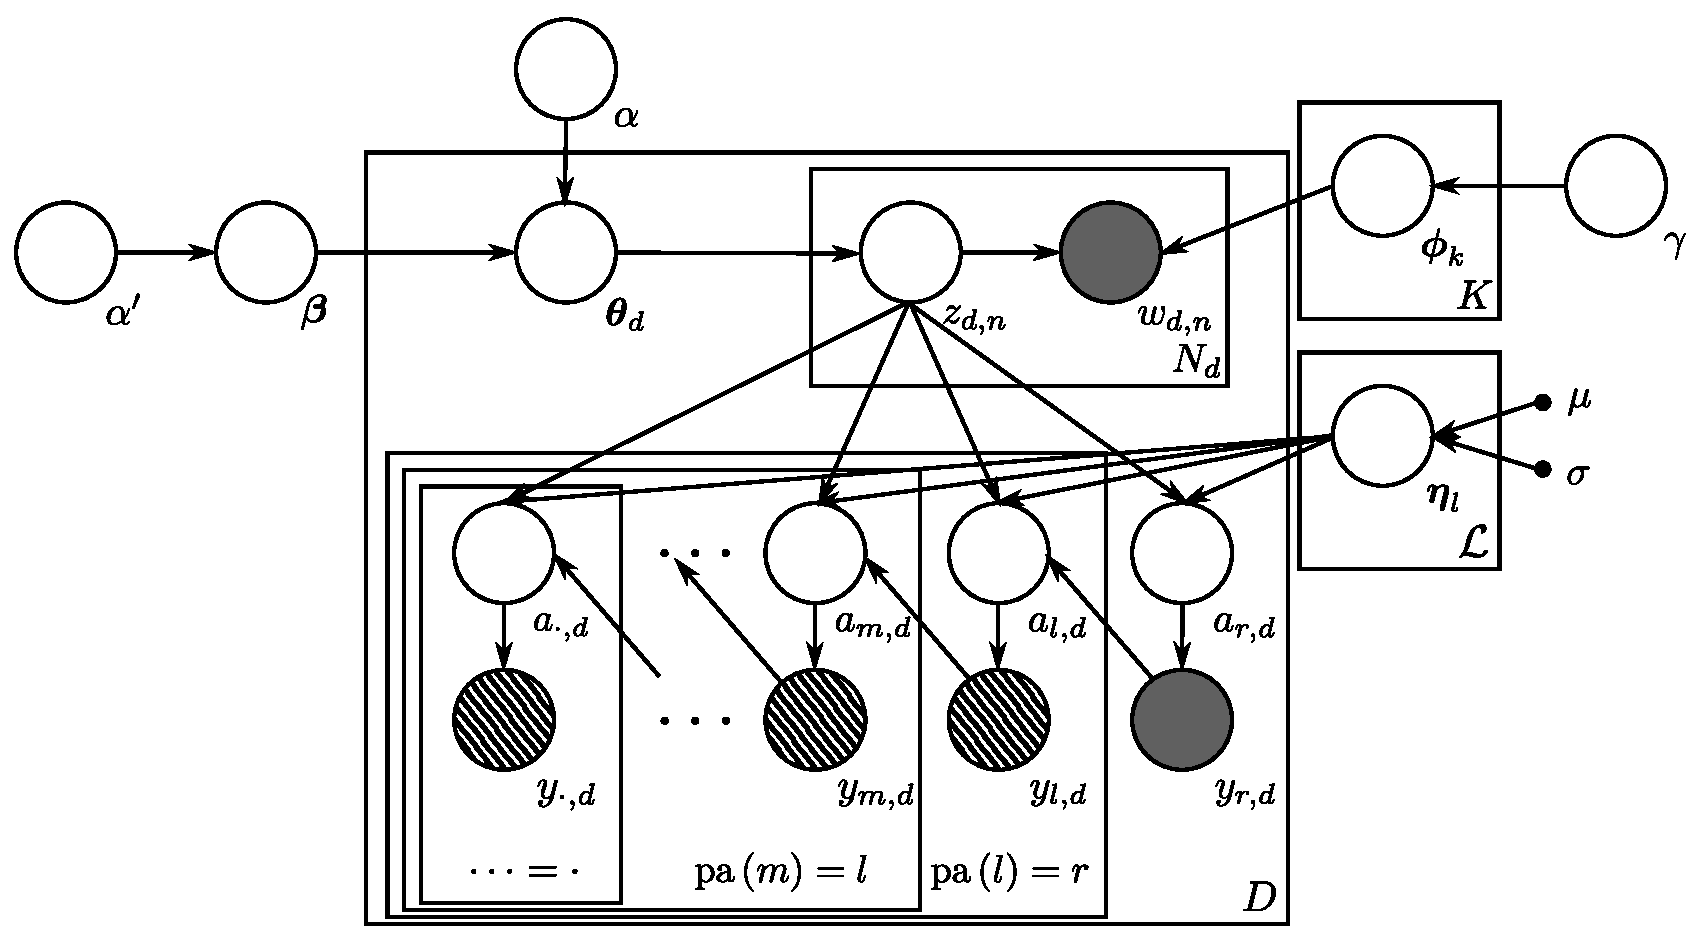
\includegraphics[scale=0.4]{Graphical_Model-final} \caption{HSLDA graphical model}


\label{fig:example} 
\end{figure}


The fixed parameters of the model are the number of topics $K$, the
number of unique words in the vocabulary $V$, the number of documents
$D$, as well as the mean, $\boldsymbol\mu$, and the standard deviation, $\sigma$,
used in a normal prior distribution. The hyper-parameters $\alpha^{\prime}$,
$\alpha$, and $\gamma$ are weight parameters for Dirichlet prior
distributions. We will denote the $K$-dimensional Dirichlet distribution
as Dir$_{K}(\cdot)$ and the $K$ dimensional normal distribution
as $\mathcal{N}_{K}(\cdot)$.

We will now describe the stochastic generative process which defines
our model. The graphical model is show in Figure~\ref{fig:example}.
%Given the number of topics, K, and broad gamma priors on hyperparameters,
%the generative process is as follows: 

\begin{enumerate}
\item For each topic $k=1,\ldots,K$

\begin{itemize}
\item Draw a distribution over words $\boldsymbol\phi_{k}\sim{\rm Dir}_{V}(\gamma\mathbf{1}_V)$%,
%where $\mathbf{1}$ is a vector of ones of length $V$ 
\end{itemize}
\item For each label $l\in\mathcal{L}$

\begin{itemize}
\item Draw a regression coefficient $\boldsymbol\eta_{l}\mid\mu,\sigma\sim\mathcal{N}_{K}(\mu \mathbf{1}_K,\sigma \mathbf{I}_{K})$,
where $\mathbf{I}_{K}$ is the $K$ dimensional identity matrix 
\end{itemize}
\item Draw the global topic proportions $\boldsymbol\beta\mid\alpha'\sim{\rm Dir}_{K}\left(\alpha^{\prime}\mathbf{1}_K\right)$
\item For each document $d=1,\ldots,D$

\begin{itemize}
\item Draw topic proportions $\boldsymbol\theta_d\mid\boldsymbol\beta,\alpha\sim{\rm Dir}_{K}\left(\alpha\boldsymbol\beta\right)$ 
\item For $n=1,\ldots,N_{d}$

\begin{itemize}
\item Draw topic assignment $z_{n,d}\mid\boldsymbol\theta_d\sim{\rm Multinomial}(\boldsymbol\theta_d)$ 
\item Draw word $w_{n,d}\mid z_{n,d},\boldsymbol\phi_{1:K}\sim{\rm Multinomial}(\boldsymbol\phi_{z_{n,d}})$ 
\end{itemize}
\item For each label $l\in\mathcal{L}$: 

\begin{itemize}
\item Draw $a_{l,d}\mid \bar{\mathbf{z}}_d,\boldsymbol\eta_{l},y_{\mathrm{pa}(l),d}\sim\begin{cases}
\mathcal{N}(\bar{\mathbf{z}}^{T}\boldsymbol\eta_{l},1), & y_{\mathrm{pa}(l)}=1\\
\mathcal{N}(\bar{\mathbf{z}}^{T}\boldsymbol\eta_{l},1)\mathbb{I}(a_{l,d}<0), & y_{\mathrm{pa}(l)}=-1\end{cases}$ \\where $\bar{z}_{d}=N_{d}^{-1}\sum_{n=1}^{N}z_{n,d}$ %\item Draw $a_{l, d} \ | \ z_{1:N_d,d}, \boldsymbol\beta_l \sim \mathcal{N} \left(\bar z_d^{T} \boldsymbol\beta_{l},1\right)$, where $\bar z_d=N_d^{-1}\sum_{n=1}^{N_d}z_{n,d}$ 
 
\item Set the response variable \[
y_{l,d}\mid a_{l,d}=\begin{cases}
\ \ \ 1 & \text{if \ensuremath{a_{l,d}>0} and \ensuremath{y_{{\rm \mathrm{pa}}(l),d}=1}}\\
-1 & \text{otherwise}\end{cases}\]
 
\end{itemize}
\end{itemize}
\end{enumerate}
This type of generative model is known as a probit regression model.
Probit regression models are a type of discriminative probabilistic
model similar to logistic regression. However, instead of using the
logistic sigmoid as the link function, the probit regression model
uses the CDF for a standard normal distribution - the inverse of which
is known as the probit. In this case, the regression is conditional
on the parents according to the constraints of the labeling hierarchy.
The latent variables $a_{l,d}$ utilized here are also known as an
auxiliary variables because the are introduced to make exact Gibbs
sampling possible and are not of primary interest.

Given that negative labels are uncommon and that the absence of a
label is not equivalent to a negative label, we apply an informative
prior to the regression parameters, $\mathbf{\boldsymbol\beta}_{\mathcal{L}}$,
in the form of a negative prior that encodes a bias towards being
truly negative in the absence of a label.

